\documentclass[a4paper,11pt]{jsarticle}
\usepackage{multirow}
%枠設定
\usepackage[margin=25mm]{geometry}
% 数式
\usepackage{amsmath,amsfonts}
\usepackage{bm}
% 画像
\usepackage[dvipdfmx]{graphicx}

\begin{document}

\section*{(1)レーザ変位計によるはりのたわみ測定}

\section{実験目的}
精密情報機器や機械要素等の設計において重要となるはりたわみについて,
レーザ式変位センサを用いて,両端支持ばりのたわみを計測することによって
理解する.

\section{はりたわみの理論}
両端支持ばりのたわみに関する模式図を図1に示す.

\begin{figure}[h]
  \centering
  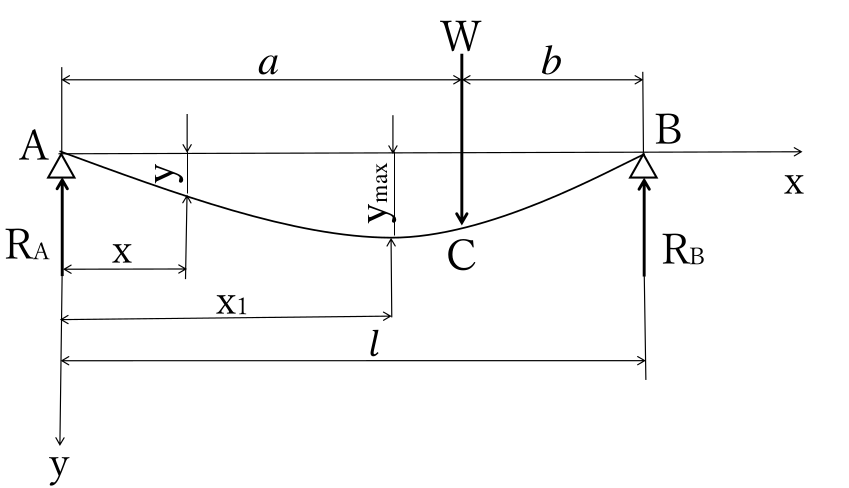
\includegraphics[width=10cm]{AB.png}
  \caption{両端支持ばりの模式図}
\end{figure}
スパン$l$の両端支持ばりABが,左支点Aから$a$,右支点Bから$b$の距離にある点Cに,集中荷重$W$を受ける場合の
最大たわみ$y_{max}$は,
\begin{equation}
  y_{max} = {\dfrac{Wb({l^2}-{b^2})^{3/2}}{9\sqrt{3}EIl}}
\end{equation}
である.ただし,最大たわみを生ずる位置$x_1$は次のようになる.
\begin{equation}
  x_1 = {\sqrt{\dfrac{a(a+2b)}{3}}}={\sqrt{\dfrac{{l^2}-{b^2}}{3}}}
\end{equation}
また,荷重点C$(x=a)$のたわみ$y_c$および中央のたわみ$(y)_{x={1/2}}$は,それぞれ
\begin{equation}
  y_{c} = {\dfrac{Wa^{2}b^{2}}{3EIl}}
\end{equation}
\begin{equation}
  (y)_{x={1/2}} = {\dfrac{Wb(3l^{2}-4b^{2})}{48EIl}}
\end{equation}
である.なお集中荷重$W$がスパンの中央に位置する場合は,
\begin{equation}
  a = b = \dfrac{1}{2}
\end{equation}
であるから,
\begin{equation}
  x_1 = \dfrac{1}{2}
\end{equation}
となり,最大たわみ$y_{max}$が求まる.
\begin{equation}
  y_{max} = {\dfrac{Wl^{3}}{48EIl}}
\end{equation}

\section{実験装置}
\begin{enumerate}
  \item はり構造の力学実験装置(青色のアングルで組まれた装置)\\
  はり\\
  支点\\
  おもり(0.500$kg$:4 個,0.200$kg$:3 個,0.100$kg$:1 個,合計 2.700$kg$)\\
  おもり支持金具(0.224$kg$)
  \item CMOS レーザアプリセンサ\\
  アンプユニット IL-1000\\
  センサヘッド IL-065\\
  電源ユニット KZ-U3
  \item マイクロメータ(最小目盛:0.001$mm$,測定範囲 0-25$mm$)
  \item マイクロメータ(最小目盛:0.001$mm$,測定範囲 25-50$mm$)
\end{enumerate}

\section{実験準備}
\begin{enumerate}
  \item CMOS レーザアプリセンサの電源ユニット KZ-U3 の電源コードをテーブルタップに接続して,
  電源投入後 30 分以上放置する.センサヘッド IL-065[基準距離:65$mm$,測定距離:55-105$mm$]
  からレーザ光(赤色半導体レーザ,可視光,波長 665$nm$)が照射される.なお,レーザ光は直接
  入らないように注意すること.
  \item アンプユニット IL-1000 測定値表示部には,センサヘッドとはり間の距離が小数点以下 3 桁まで
  表示される(単位 $mm$).表示が安定しない場合は,センサヘッドのフィルタガラスが汚れている
  可能性があるため,柔らかい布で拭きとる.
\end{enumerate}

\section{実験方法}
\begin{enumerate}
  \item はりの断面の幅 $b'$,高さ $h$ を左右支点近傍と中央の 3 箇所について,マイクロメータを使って
  小数点以下 3 桁まで測定する.\\
  \quad 断面二次モーメント $I$ は,次式で求められる.
  \begin{equation}
    I = {\dfrac{b'h^3}{12}}
  \end{equation}
  \item スパンの長さ$ l $は,$l= 800[mm] $である.
  \item まずは,左支点 A から集中荷重$ W $の作用点 C までの距離を$a = 500[mm] $とする.
  \item 左支点 A から最大たわみ$y_{max}$を生ずる位置までの距離 $x_1$[$mm$] を式 (2) から求める.
  \item 左支点 A から $x_1$ の位置にセンサヘッド支持台中心を移動させ,はりに対して下側からレーザ光を照射する.
  センサの動作確認 LED ではりとの距離を調整し,測定面に対してセンサの投光面が平行になるように
  設定して固定する.緑 LED が点灯しているときは,はりがセンサの測定範囲に位置しており,測定が可能である.
  \item  集中荷重 $W$ の作用点 $C$ におもり支持金具を取りつける.
  \item アンプユニット IL-1000 の ZERO SHIFT スイッチを押して,表示を ”0.000” にする.\\
  はりにおもり支持金具の重さ(0.224$kg$)の荷重がかかったところが基準になることに,注意すべきである.
  \item はりに荷重を載せていくと,荷重の増加とともにはりとセンサヘッド間の距離が減少する.
  荷重を 0[$kg$] から順に 0.5,1.0,1.5,2.0,2.2,2.4,2.6,2.7[$kg$]と増加させていき,それぞれの
  荷重に対応する最大たわみ$y_{max}$を記録する.
  \item 荷重を 2.7[$kg$]から順に 2.6,2.4,2.2,2.0,1.5,1.0,0.5,0[$kg$]と減少させていき,それぞれの
  荷重に対応する最大たわみ$y_{max}$を記録する.
  \item つぎに,$a= 600[mm],700[mm]$のそれぞれの場合について,4から9までを繰り返す.
\end{enumerate}

\section{実験結果の整理}
・はりのスパン:$l = 800[mm]$\\
\quad・鋼の縦弾性係数(標準値):
\begin{equation} 
  E = 2.06 \times 10^5 [MPa] 
\end{equation}

\begin{enumerate}
  \item はり断面の幅 $b'$ と高さ $h$ を表 1 に記録する.
  \item $a = 500 [mm] $のとき,最大たわみ$y_{max}$ を生ずる位置 $x_1$ は$ 428.2 [mm]$ である.
  荷重を増加させたときの最大たわみ $(y_{max})_i$と,減少させたときの最大たわみ $(y_{max})_d$を,表2
  に記録する.最大たわみの理論値 $y_{max}$は,式 (1) から計算する.また,誤差率$ \delta [\%]$は,
  \begin{equation} 
    \delta = \frac{{\left(\frac{{(y_{\text{max}})_i + (y_{\text{max}})_d}}{2} - y_{\text{max}}\right)}}{{y_{\text{max}}}} \times 100[\%]
  \end{equation}
  から計算する.
  \item $a = 600 [mm] $のとき,最大たわみ$ y_{max}$を生ずる位置 $x_1$は $447.2 [mm] $である.
  2と同様にして,表3に最大たわみ$y_{max}$の値を記録する.
  \item $a = 700 [mm] $のとき,最大たわみ$ y_{max}$を生ずる位置 $x_1$は $458.3 [mm] $である.
  2と同様にして,表4に最大たわみ$y_{max}$の値を記録する.
\end{enumerate}

% ページ1の挿入
\begin{figure}[htbp]
  \centering
  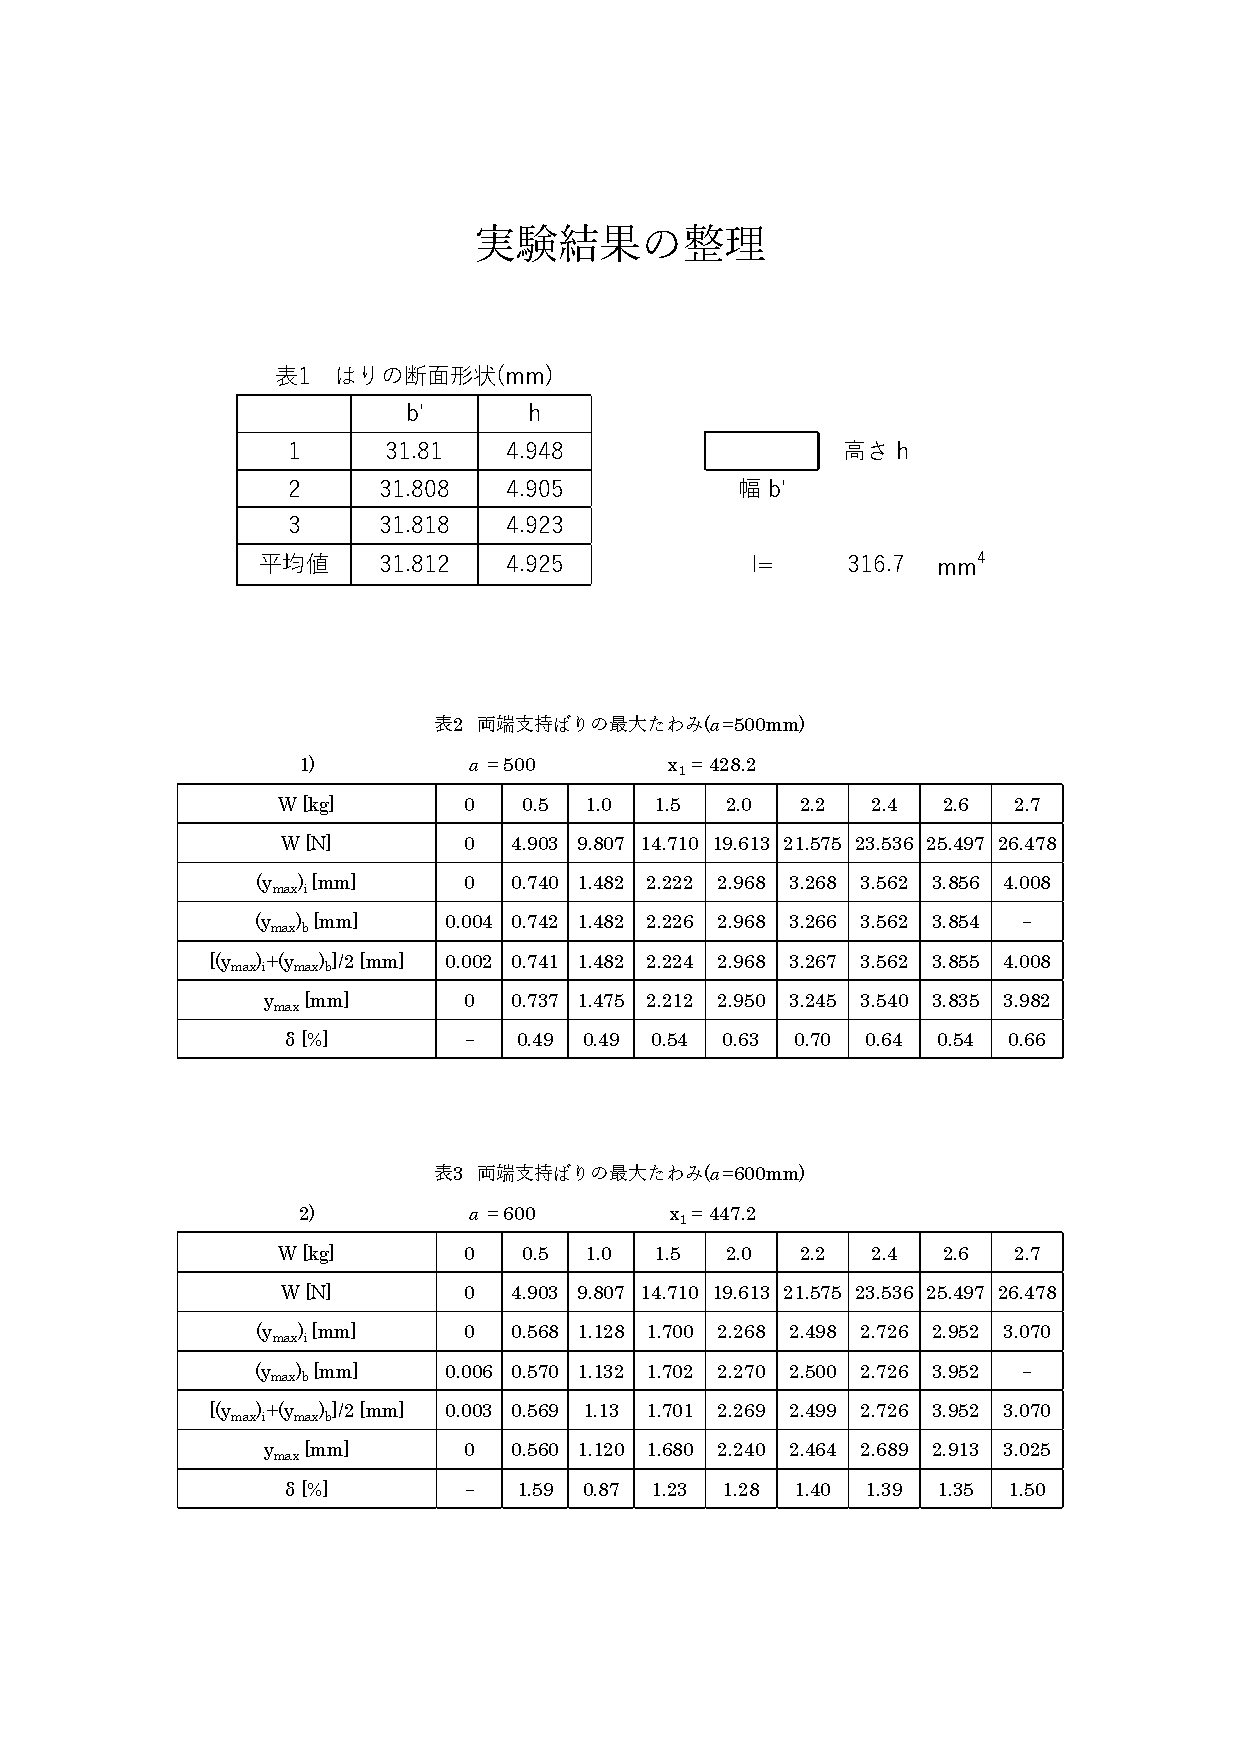
\includegraphics[page=1,width=\textwidth,height=\textheight]{1.pdf}
\end{figure}

\clearpage

% ページ2の挿入
\begin{figure}[htbp]
  \centering
  \includegraphics[page=2,width=\textwidth,height=\textheight]{1.pdf}
\end{figure}
\clearpage

\section{考察および課題}
\begin{enumerate}
  \item 図1の左支点 $A$から集中荷重$ W$ の作用点 $C $までの距離 $a$ が $500,600,700 [mm]$と増加するに
  つれて,$x_1$ はどのように変化するか.図(横軸を $a $,縦軸を$x_1$とする) を描き,考察せよ.[図2]\\
  \\
  \quad 図2は,横軸を$a$,縦軸を$x_1$として$a$と$x_1$の関係をグラフで示している.
  図2から明らかなように,左支点Aから点Cまでの距離が増加すると,最大たわみを生じる$x_1$も増加する.
  また,式(2)の$l^2-b^2$の$b$の値が小さくなると,$x_1$が大きくなることからも,
  実験結果の正当性が裏付けられる.
\clearpage
\begin{figure}[h]
  \centering
  \rotatebox{90}{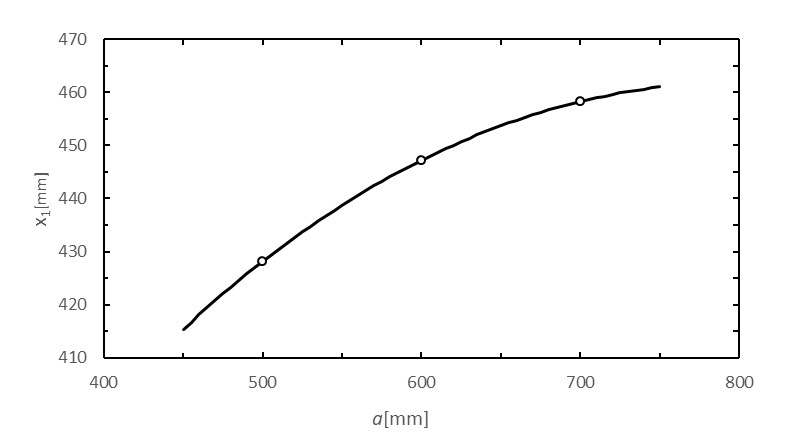
\includegraphics[width=25cm]{1.jpg}}
  \caption{$a$と$x_1$の関係}
\end{figure}
\clearpage
\item 横軸に荷重 $W [N] $を,縦軸に最大たわみ$ y_{max}[mm]$(測定値および理論値)をとり,$a$ を変化さ
せた図を描け[図3~5].\\
図3~5を 1 つの図にまとめよ[図6].\\
横軸に$ W [N]$を,縦軸に誤差率$ \delta [\%]$をとって,図を描け[図7].\\
実験結果(図3~7)について,それぞれ考察せよ.\\
  
\quad 図3から5に$a = 500,600,700$ のときの,荷重$ W [N] $と,最大たわみ $y_{max}$の関係をグラフを示す.
図6に$a = 500,600,700$ をまとめたものを示す.図7に軸に$ W [N]$を,縦軸に誤差率$ \delta [\%]$を
取ったものを示す.図3から5より測定値が理論値を大きく外れていないことが確認できる.また荷重 $W [N] $と最大たわみ$ y_{max}[mm]$
が比例関係にあることも直線であることから読み取れる.図6より$a$が大きくなればなるほど傾きが小さくなっているのがわかる.
これは端によれば寄るほど最大たわみが小さくなることを示している.
誤差の原因として考えられるのは,おもりを置くときの過失誤差似用影響が大きいと考える.
式(1)の$b$を$l-a$とすると$a$が大きくなれば分母が小さくなり$y_{max}$が小さくなることがわかる.
図7より誤差率は$a$が大きいほど高くなっている.
図1より垂直方向の力のつり合いと B 点に関するモーメントのつり合いから,
\begin{equation} 
  R_A+R_B=W,R_al-W(l-a)=0
\end{equation}
となり,これから
\begin{equation} 
  R_A={\dfrac{l-a}{l}W},R_B={\dfrac{a}{l}W}
\end{equation}
を得る.$x$断面における曲げモーメントは,AC 側と CB 側とでは,
\begin{equation} 
  M_{AC}=R_Ax={\dfrac{W(l-a)}{l}x},M_{CB}=R_Ax-W(x-a)={\dfrac{Wa}{l}(l-x)}
\end{equation}
となる.したがって,たわみの基本式より
\begin{equation} 
  {(\dfrac{d^2y}{dx^2})_{AC}}={-\dfrac{W(l-a)}{EIl}x},
  {(\dfrac{d^2y}{dx^2})_{CB}}={-\dfrac{Wa}{EIl}(l-x)}
\end{equation}
となる.これを積分すれば
\begin{equation} 
  {(\dfrac{dy}{dx})_{AC}}={-\dfrac{W(l-a)}{2EIl}x^2+c_1},
  {(y)_{AC}}={-\dfrac{W(l-a)}{6EIl}x^3+c_1x+c_2}
\end{equation}

\begin{equation} 
{(\dfrac{dy}{dx})_{CB}}={-\dfrac{Wa}{EIl}(lx-\dfrac{1}{2}x)+c_1},
{(y)_{CB}}={-\dfrac{Wa}{EIl}(\dfrac{l}{2}x^2-\dfrac{1}{6}x^3)+c_3x+c_4}
\end{equation}
となる.しかるに$x=0$で$y=0$であるため,$c_2=0$,また$x=l$で$y=0$であるため,
\begin{equation} 
  {-\dfrac{Wal^2}{3EIl}+c_3l+c_4}=0
  \end{equation}
  となる.一方で,$x=a$においては両側のたわみ角とたわみが等しく
  \begin{equation} 
    c_4={-\dfrac{Wa^3}{6EI}}
  \end{equation}
となる.これを式(17)にいれ計算すると
\begin{equation} 
  c_3={\dfrac{Wa}{6EIl}(2l^2+a^2)}
\end{equation}
\begin{equation} 
  c_1={\dfrac{W(l-a)}{6EIl}(2la-a^2)}
\end{equation}
となる.これら積分定数も値をもとに計算すると


\clearpage
\begin{figure}[h]
  \centering
  \rotatebox{90}{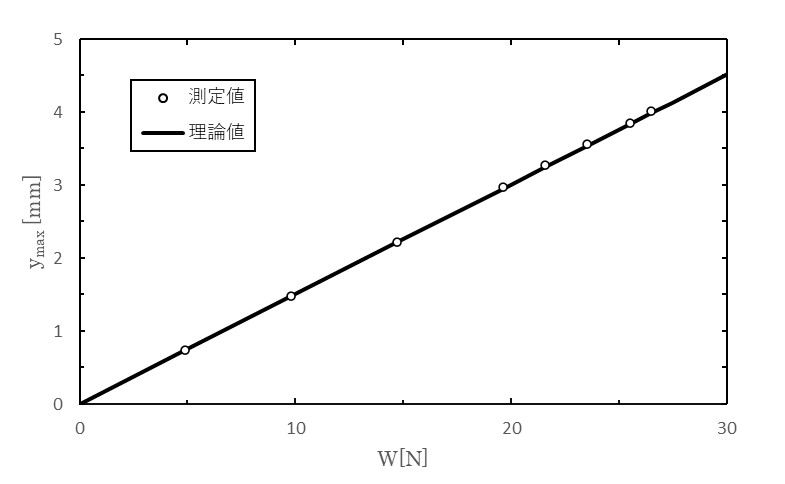
\includegraphics[width=23.5cm]{2.jpg}}
  \caption{$a = 500$}
\end{figure}
\clearpage
\begin{figure}[h]
  \centering
  \rotatebox{90}{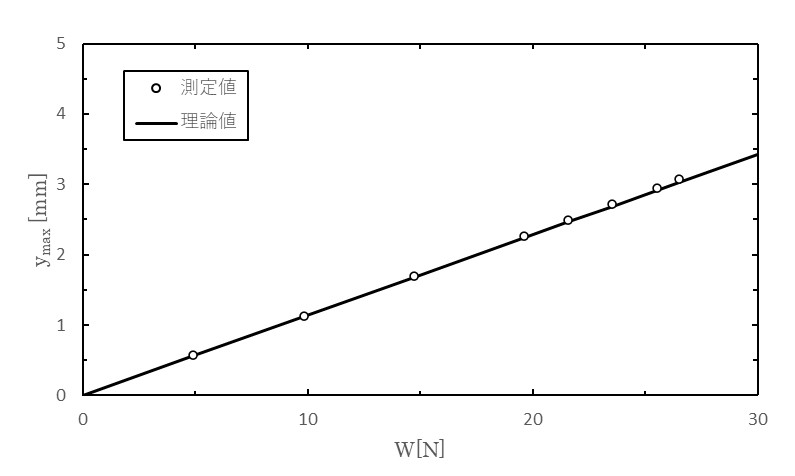
\includegraphics[width=24cm]{3.jpg}}
  \caption{$a =600$}
\end{figure}
\clearpage
\begin{figure}[h]
  \centering
  \rotatebox{90}{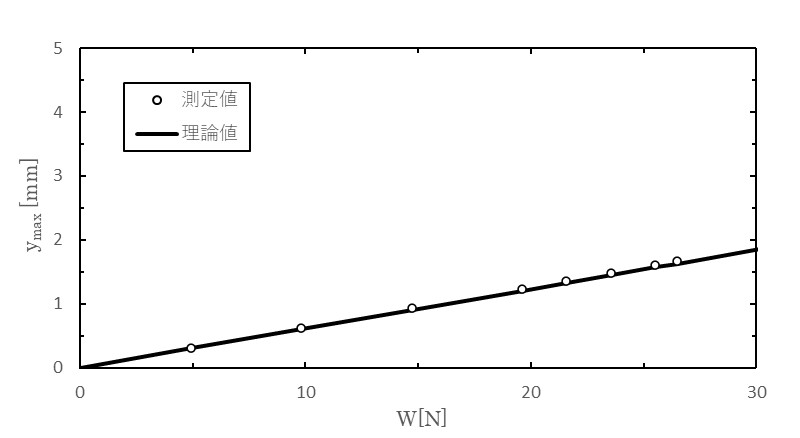
\includegraphics[width=24cm]{4.jpg}}
  \caption{$a = 700$}
\end{figure}
\clearpage
\begin{figure}[h]
  \centering
  \rotatebox{90}{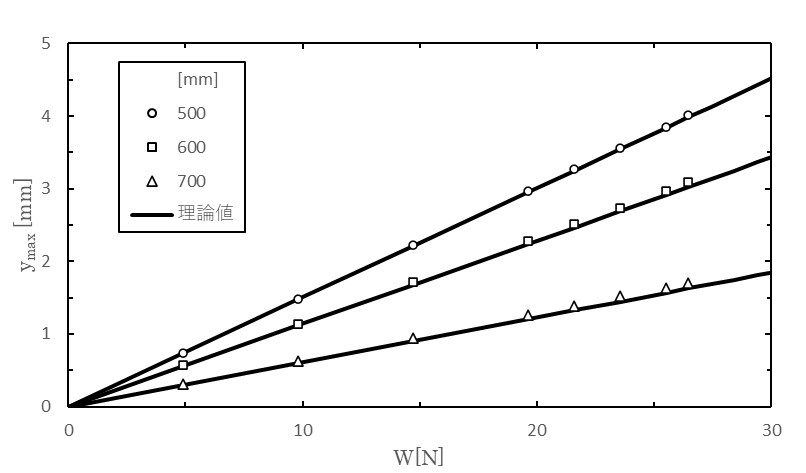
\includegraphics[width=24cm]{5.jpg}}
  \caption{$a = 500,600,700$}
\end{figure}
\clearpage
\begin{figure}[h]
  \centering
  \rotatebox{90}{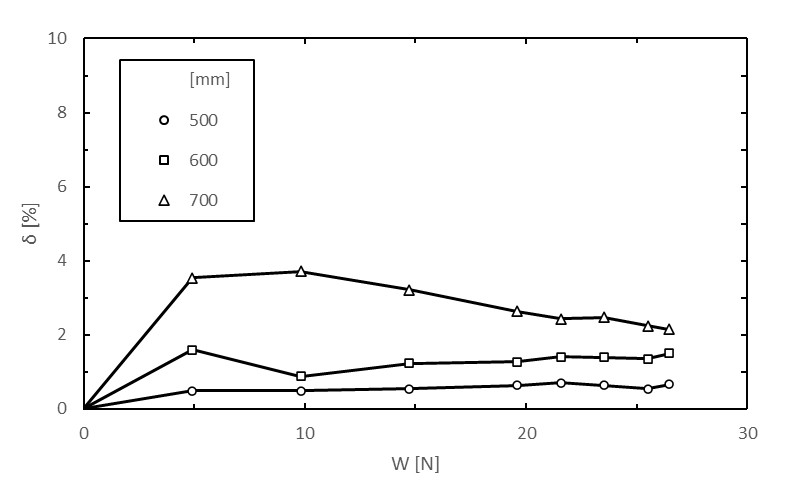
\includegraphics[width=24cm]{6.jpg}}
  \caption{荷重と誤差率}
\end{figure}
\clearpage
\item レーザの特徴およびその応用技術について,くわしく説明せよ.\\
\quad レーザ(LASER)は,"Light Amplification by Stimulated Emission of Radiation" 
の略称であり,光の増幅と刺激放射による放射を利用した装置である.レーザは光子の刺激放射を利用して光を増幅する.
レーザ媒質内にエネルギーを供給することで,媒質内の原子や分子の励起状態を
作り出す.励起された原子や分子は,外部からの光子の刺激によってエネルギーを放出し,さらに光子を放出する.
この放出された光子は,他の励起された原子や分子に対して刺激を与え,同様の光子の放出を引き起こす.
このプロセスが連鎖的に繰り返されることで,光が増幅され,高強度・高集束・単色性を持つレーザ光が生成される$^{[2]}$.
表1にレーザの種類と特徴を示す$^{[3]}$.\\レーザ媒質によって波長や特徴が大きく変わるのが確認できる.


\begin{table}[h]
  \caption{レーザの種類と特徴}
  \small % 表全体のフォントサイズを縮小するために \small を追加
  \begin{tabular}{|p{1cm}|p{2cm}|p{5cm}|p{4.5cm}|p{3cm}|}
  \hline
                      相変化   &  相変化 &  レーザ媒質  &   発振波長 &   動作モード        \\ \hline
  \multicolumn{1}{|l|}{気体} & 混合ガス   & COレーザ,$CO_2$レーザ ,色素レーザ  &$500nm,10.6{\textmu}m,320〜1260nm$ &CW,パルス  \\ \cline{3-5} 
  \multicolumn{1}{|l|}{} &    &エキシマレーザ ArF,KrF,XeCl  & $193,248,308nm$ & パルス \\ \hline
  \multicolumn{1}{|l|}{液体} &  有機系 &  色素レーザ  & $320〜1260nm$ & CW,パルス      \\ \hline
  \multicolumn{1}{|l|}{個体} &  結晶体& ルビーレーザ,チタンファイヤレーザ,YVO4,YAG & $684.3,800,1064,1064nm $  &  パルス,CW      \\ \cline{2-5} 
  \multicolumn{1}{|l|}{} & アモルファス& ガラスレーザ & $1060nm$  & パルス  \\ \cline{2-5} 
  \multicolumn{1}{|l|}{} &  半導体&AlGaAsp,InGaAsP,ZnSe &$700〜900nm,1〜1.6{\textmu}m,490nm$ & CW  \\ \cline{2-5} 
  \multicolumn{1}{|l|}{} & ファイバー & $Nd^{3+},Er^{3+},Yd^{3+}$ &$1060,1540,1030〜2200nm$ & CW \\ \hline
  \end{tabular}
  \end{table}
ではどのようなところでレーザが使われているのか,
応用例として実際に触ったことがあるレーザー加工機とLIDERについて詳しく述べる.
\quad レーザー加工は,レーザーの高いエネルギー密度を利用して,材料の切断だけでなく,溶接,穴あけなどを
行う加工技術である.一般的には炭酸ガスレーザやYAGレーザ,エキシマレーザなどが使われる.
金属を加工する場合は主に炭酸ガスレーザ,YAGレーザが使用される.厚さにもよるが硬いダイヤモンドでも
ドリルより圧倒的に早く穴を開けることができる.
今後,ダイヤモンド半導体などのダイヤモンド加工には必須の技術であると言えるだろう.
\quad 次に,LIDARについて説明する.
LIDARは,レーザー光を照射して,その反射光の情報をもとに対象物までの距離や対象物の形などを
計測する技術のことでL自律走行車やロボットなどのセンシング技術として広く使用されている.
LIDARは,環境をスキャンして三次元の地図を作成するためにも使用され,この技術はSLAM
(Simultaneous Localization and Mapping)などの応用に必要不可欠である.
図8に,私が実際に2DLIDARを使用して自分の寮の部屋をスキャンした際の様子を示す.
このデータはROS(Robot Operating System)を使用してセンサーデータを読み取り表示させたものである.
なお,実際の自動運転車や配膳ロボットなどでは,3DLIDARが使用されることが多い.
今後,自動運転や自動ロボットなどで活躍することが期待される.

\begin{figure}[h]
  \centering
  \rotatebox{90}{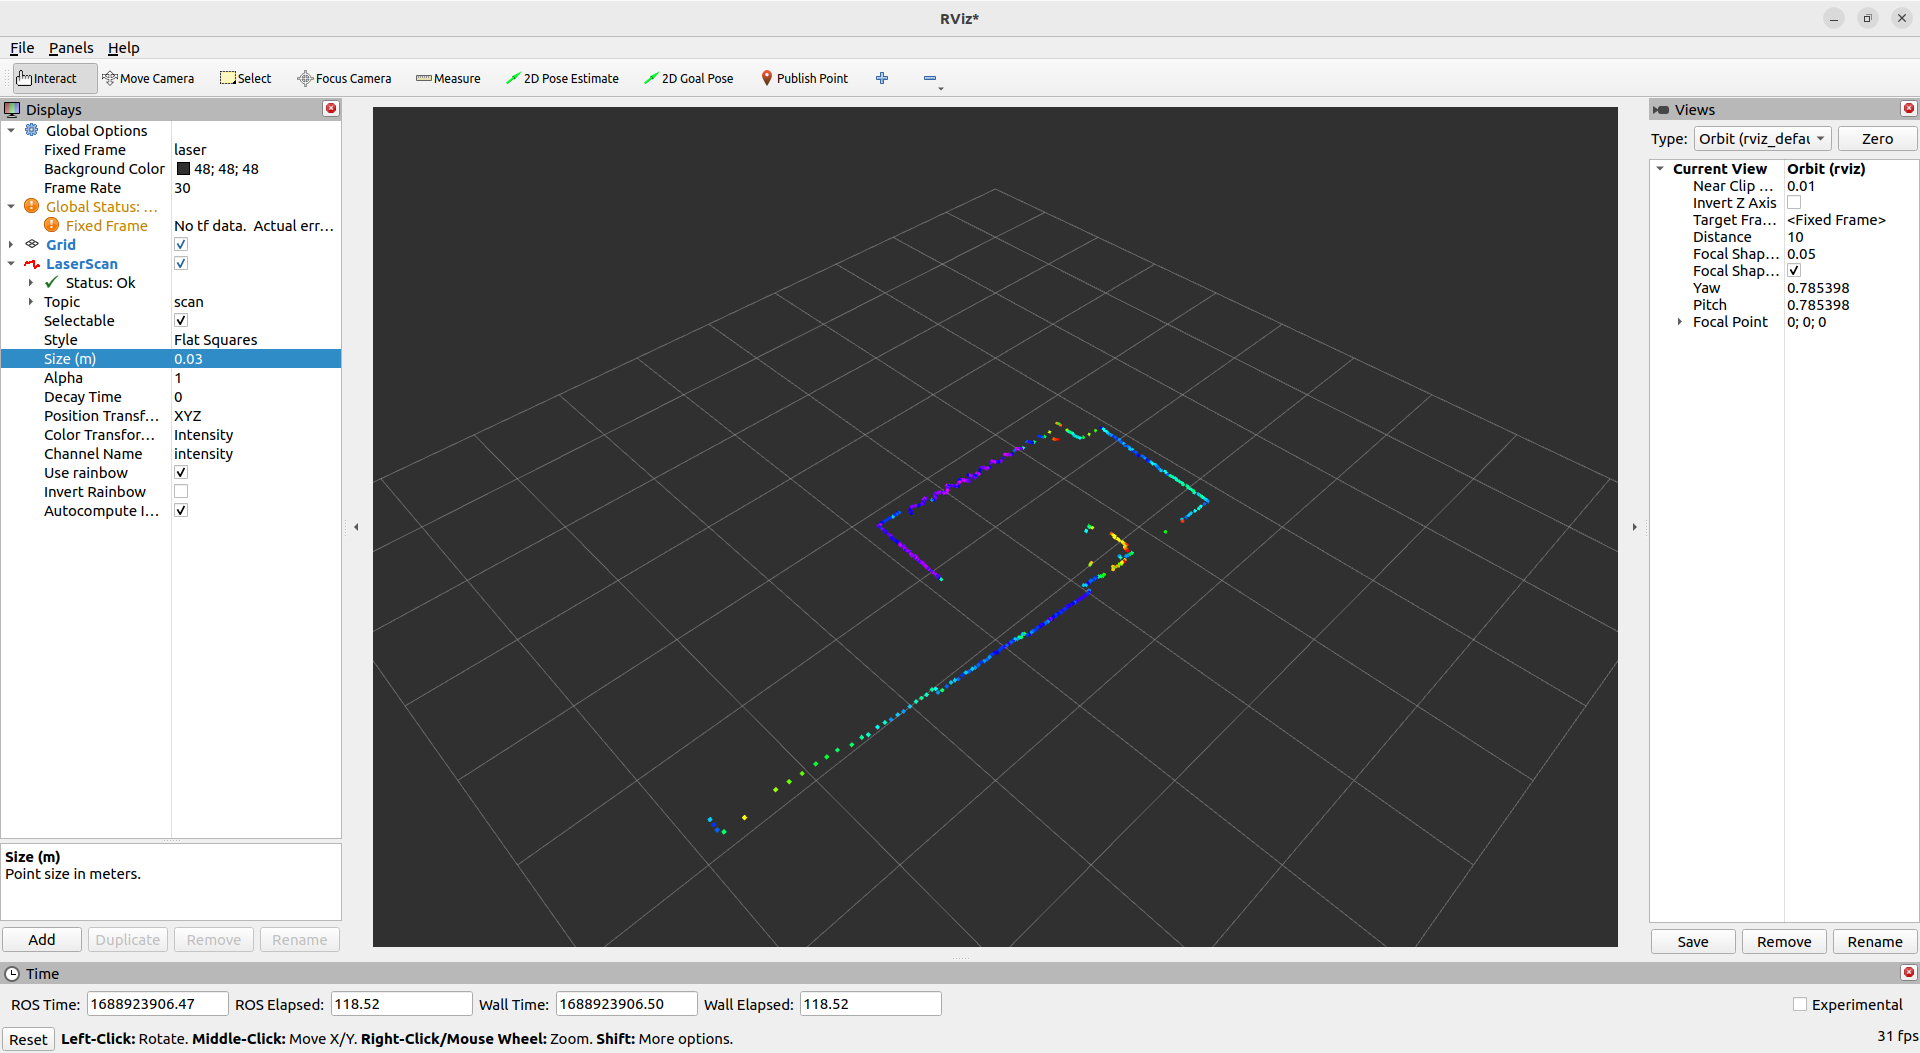
\includegraphics[width=24cm]{7.png}}
  \caption{LIDER}
\end{figure}
\clearpage
\item 精密情報機器の設計にははりのたわみの概念が重要になっている.具体例を挙げて,くわしく説明
せよ.\\
\quad はりのたわみとは,はりが荷重を受けて変形した状態のとき,
初期のはりのラインが湾曲した曲線をいう.はりのたわみは,弾性曲線方程式という微分方程式で
表される.精密情報機器の設計においては,はりのたわみを考慮することで,部品の寸法や材料の選定を行う必要がある.
具体例として,CDプレーヤーやブルーレイディスクにおけるピックアップヘッドの位置決めにはりのたわみが
関係している.ピックアップヘッドは,ディスク上の微細な凹凸をレーザー光で読み取る装置である.
ピックアップヘッドは,ディスクと一定の距離を保ちながら,高速で回転するディスクに追従する必要がある.
このとき,ピックアップヘッドを支える部品(アームやばねなど)がはりとして振る舞い,
荷重や振動によってたわみが生じる.このたわみが大きくなると,ピックアップヘッドとディスクの距離が変化し,
読み取りエラーや音飛びなどの不具合が発生する可能性がある.
したがって,CDプレーヤーやブルーレイディスクの設計においては,
ピックアップヘッドを支える部品のたわみを最小限に抑えることが重要である.
これには,部品の形状や寸法を適切に設計することや,弾性率や密度などの材料特性を考慮することが必要であるといえる$^{[4]}$$^{[5]}$$^{[6]}$$^{[7]}$$^{[8]}$.
\begin{figure}[h]
  \centering
  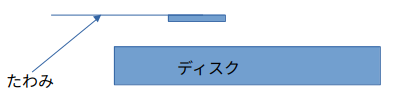
\includegraphics[width=10cm]{8.png}
  \caption{LIDER}
\end{figure}

\end{enumerate}

\begin{thebibliography}{20}
  \bibitem{} 
  中山 秀太郎:演習・材料力学入門,大河出版(2007),p.122-124
  \bibitem{} 
  谷腰 欣司:レーザー技術入門講座,電波新聞社(2007),p.51 -63
  \bibitem{}
  谷腰 欣司:レーザー技術入門講座,電波新聞社(2007),p.87
  
  \bibitem{}
  弾性曲線方程式 - Wikipedia https://ja.wikipedia.org/wiki/ (2023/07/08)
  \bibitem{} 
  ブルーレイディスクのしくみ | ブルーレイディスクとは | ブルーレイディスクレコーダー | ソニー https://www.sony.jp/bd/about/technology/ (2023/07/08)
  \bibitem{} 
  CDプレーヤーの寿命は?何年持つ? https://rank-king.jp/article/7648 (2023/07/08)
  \bibitem{}
  佐藤卓蔵:レーザ[CD プレーヤから X 線レーザまで],電気書院(1997),p.134
  \bibitem{}
  はりのたわみ(機械工学と自動機設計-17) | 技術情報 | MISUMI-VONA【ミスミ】(2023/07/08)
\end{thebibliography}


\end{document}